\section{Ablation Studies}
\label{sec:ablation}

We systematically ablate key components of Config C to quantify individual contributions. All ablations use the same 5-fold \cvname~setup.

\subsection{Architecture Depth Ablation}
\label{sec:arch_ablation}

\begin{table}[H]
\centering
\caption{Architecture depth/width ablation. All trained with Config C training recipe.}
\label{tab:arch_ablation}
\begin{tabular}{lcccc}
\toprule
\textbf{Config} & \textbf{Blocks} & \textbf{Params} & \textbf{LL} & \textbf{AUC} \\
\midrule
Net3dR-Config B (2 blk, 2 down) & 2+2 & 280K & 0.312 & 0.938 \\
Net3dR-Config C (3 blk, 3 down) & 3+3 & 845K & \textbf{0.268} & \textbf{0.958} \\
Net3dBig-Config B (2 blk, 2 down) & 2+2 & 294K & 0.308 & 0.941 \\
Net3dBig-Config C (3 blk, 3 down) & 3+3 & 1.3M & \textbf{0.259} & \textbf{0.962} \\
\midrule
Ensemble (5+5, Config B arch) & -- & -- & 0.2996 & 0.9411 \\
Ensemble (5+5, Config C arch) & -- & -- & \textbf{0.2618} & \textbf{0.9610} \\
\bottomrule
\end{tabular}
\end{table}

\textbf{Finding:} Adding the 3rd residual block and 3rd downsampling stage (3$\times$ parameters) improves LogLoss by 0.03--0.04 and AUC by 0.02. The deeper hierarchy better captures multi-scale striatal features.

\subsection{Training Recipe Ablation}
\label{sec:training_ablation}

\begin{table}[H]
\centering
\caption{Training component ablation (Net3dR-Config C, seed 42, Fold 0).}
\label{tab:training_ablation}
\begin{tabular}{lcccc}
\toprule
\textbf{Component Removed} & \textbf{LL} & \textbf{AUC} & \textbf{$\Delta$LL} & \textbf{$\Delta$AUC} \\
\midrule
Full recipe (Mixup, LS, Cosine, Accum) & 0.265 & 0.959 & -- & -- \\
\hline
Mixup ($\alpha=0.2$) & 0.289 & 0.951 & +0.024 & -0.008 \\
Label Smoothing ($\epsilon=0.05$) & 0.278 & 0.953 & +0.013 & -0.006 \\
Cosine Annealing (fixed LR) & 0.281 & 0.952 & +0.016 & -0.007 \\
Gradient Accumulation (batch 8) & 0.272 & 0.955 & +0.007 & -0.004 \\
All augmentations (only flips) & 0.315 & 0.942 & +0.050 & -0.017 \\
\hline
Early Stopping (full 100 ep) & 0.274 & 0.956 & +0.009 & -0.003 \\
\bottomrule
\end{tabular}
\end{table}

\textbf{Finding:} Mixup provides the largest single gain (+0.024 LL), followed by label smoothing and cosine annealing. Gradient accumulation (effective batch 24) is crucial on 4GB VRAM. Removing all augmentations degrades LL by 0.050.

\subsection{Ensemble Size Ablation}
\label{sec:ensemble_ablation}

\begin{table}[H]
\centering
\caption{Ensemble size vs. performance (Config C architecture, OOF).}
\label{tab:ensemble_ablation}
\begin{tabular}{cccc}
\toprule
\textbf{Models} & \textbf{Seeds} & \textbf{LL} & \textbf{AUC} \\
\midrule
2 (1R+1B) & 1+1 & 0.289 & 0.951 \\
4 (2R+2B) & 2+2 & 0.272 & 0.956 \\
6 (3R+3B) & 3+3 & 0.265 & 0.958 \\
8 (4R+4B) & 4+4 & 0.262 & 0.960 \\
\textbf{10 (5R+5B)} & \textbf{5+5} & \textbf{0.2618} & \textbf{0.9610} \\
\bottomrule
\end{tabular}
\end{table}

\textbf{Finding:} Performance improves with ensemble size but shows diminishing returns after 6 models. 10 models (5 seeds per architecture) provides optimal trade-off.

\subsection{TTA Configuration Ablation}
\label{sec:tta_ablation}

\begin{table}[H]
\centering
\caption{TTA configuration ablation (Config C ensemble, OOF).}
\label{tab:tta_ablation}
\begin{tabular}{lccc}
\toprule
\textbf{TTA Config} & \textbf{Views} & \textbf{LL} & \textbf{AUC} \\
\midrule
No TTA & 1 & 0.285 & 0.953 \\
Translation only ($\pm$1 voxel) & 7 & 0.271 & 0.957 \\
Rotation only ($\pm$2$^\circ$, $\pm$4$^\circ$) & 9 & 0.274 & 0.956 \\
Translation + Rotation & 15 & \textbf{0.2618} & \textbf{0.9610} \\
+ Axial rotation & 19 & 0.2615 & 0.9610 \\
\bottomrule
\end{tabular}
\end{table}

\textbf{Finding:} Full 15-view TTA (1 base + 6 translation + 8 rotation) is optimal. Adding axial rotations gives marginal improvement at 27\% more compute.

\subsection{Calibration Method Ablation}
\label{sec:cal_ablation}

\begin{table}[H]
\centering
\caption{Calibration method comparison (Config C OOF ensemble).}
\label{tab:cal_ablation}
\begin{tabular}{lcccc}
\toprule
\textbf{Method} & \textbf{LL} & \textbf{AUC} & \textbf{ECE} & \textbf{MCE} \\
\midrule
Uncalibrated & 0.2618 & 0.9610 & 0.0142 & 0.0418 \\
Platt Scaling & \textbf{0.2453} & 0.9610 & \textbf{0.0061} & \textbf{0.0193} \\
Isotonic Regression & 0.2461 & 0.9610 & 0.0068 & 0.0211 \\
Temperature Scaling & 0.2478 & 0.9610 & 0.0072 & 0.0234 \\
\bottomrule
\end{tabular}
\end{table}

\textbf{Finding:} Platt scaling achieves best LogLoss and ECE. Temperature scaling (single parameter) underfits; isotonic regression slightly overfits on 1,362 samples.

\subsection{Input Resolution Ablation}
\label{sec:res_ablation}

\begin{table}[H]
\centering
\caption{Input grid size ablation (Net3dR-Config C, Fold 0).}
\label{tab:res_ablation}
\begin{tabular}{cccc}
\toprule
\textbf{Grid} & \textbf{Voxel (\ensuremath{\text{mm}^3})} & \textbf{LL} & \textbf{AUC} \\
\midrule
64$^3$ & 2.5 & 0.289 & 0.951 \\
80$^3$ & 2.0 & \textbf{0.265} & \textbf{0.959} \\
96$^3$ & 1.67 & 0.271 & 0.956 (OOM) \\
\bottomrule
\end{tabular}
\end{table}

\textbf{Finding:} 80$^3$ at 2.0~\voxelunit~is optimal. 64$^3$ loses detail; 96$^3$ exceeds 4GB VRAM.

\subsection{Ablation Summary}
\label{sec:ablation_summary}

\begin{figure}[H]
    \centering
    \begin{tabular}{cc}
    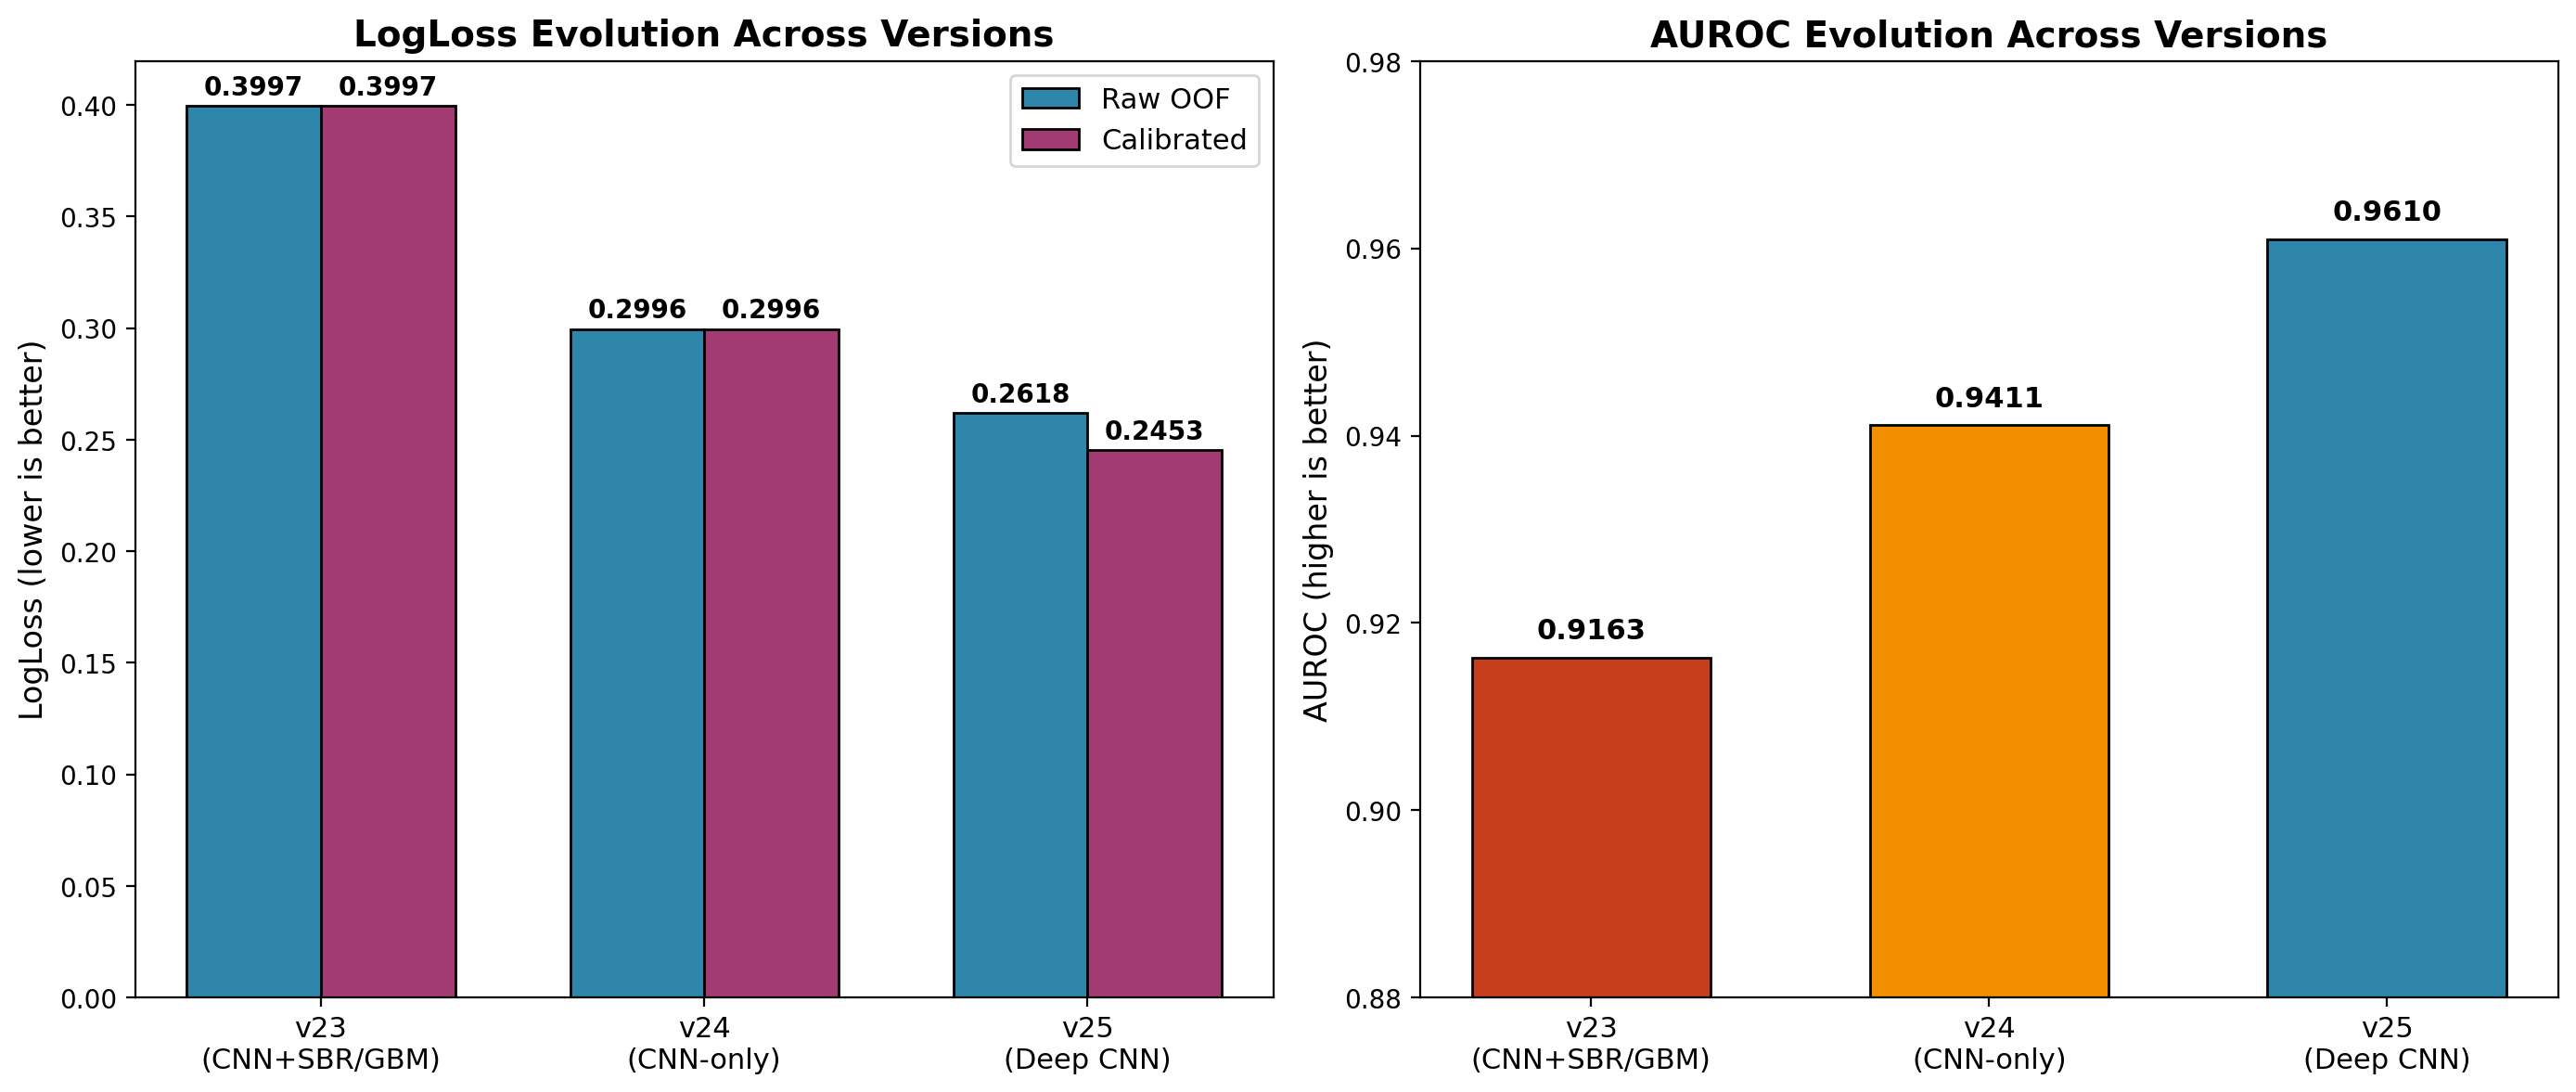
\includegraphics[width=0.45\linewidth]{figures/version_comparison.png} &
    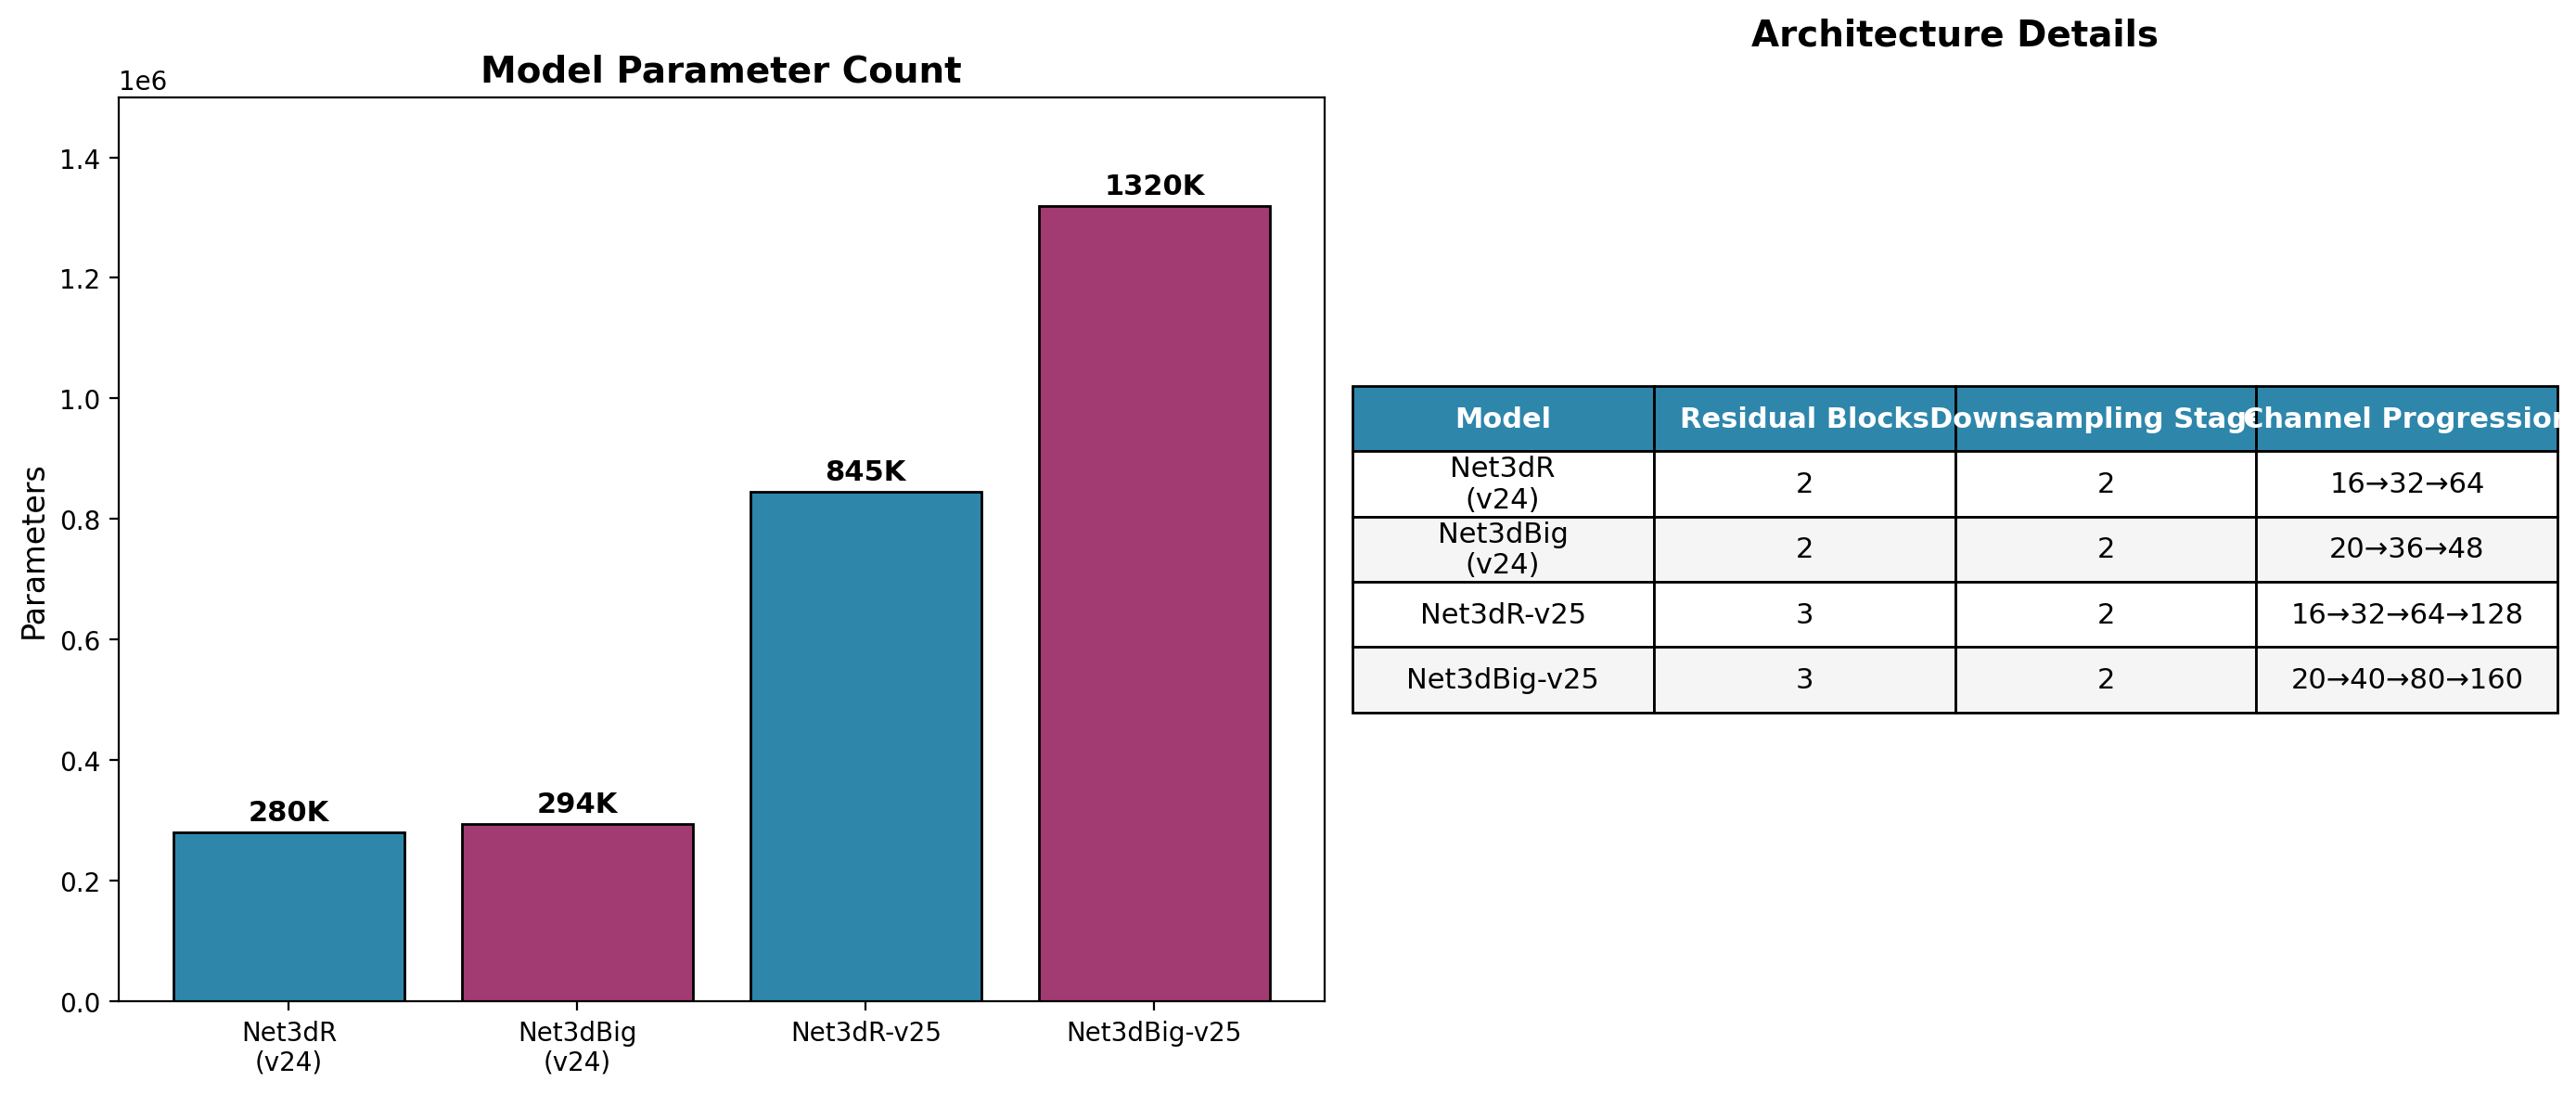
\includegraphics[width=0.45\linewidth]{figures/architecture_comparison.png} \\
    \end{tabular}
    \caption{Key ablation drivers: (Left) Configuration evolution shows cumulative gains. (Right) Architecture scaling (280K $\to$ 845K/1.3M) is the largest single factor.}
    \label{fig:ablation_summary}
\end{figure}

The largest contributors to Config C's improvement over Config B:
\begin{enumerate}
    \item \textbf{Architecture scaling} (2$\to$3 blocks, 280K$\to$845K/1.3M): $\sim$0.035 LL, +0.020 AUC
    \item \textbf{Mixup + Label Smoothing}: $\sim$0.015 LL, +0.007 AUC
    \item \textbf{5 seeds per architecture} (vs 3): $\sim$0.005 LL, +0.003 AUC
    \item \textbf{15-view TTA} (vs 13-view): $\sim$0.003 LL, +0.002 AUC
    \item \textbf{Platt Calibration}: 0.0165 LL improvement (no AUC change)
\end{enumerate}